% Prof. Dr. Ausberto S. Castro Vera
% UENF - CCT - LCMAT - Curso de Ci\^{e}ncia da Computa\c{c}\~{a}o
% Campos, RJ,  2023
% Disciplina: An\'{a}lise e Projeto de Sistemas
% Aluno: Rômulo Souza Fernandes

\chapterimage{planejamento.png} % Table of contents heading image
\chapter{Etapa de Planejamento}


Neste capítulo é apresentado o ciclo de vida do desenvolvimento de sistemas, onde as bases do projeto são estabelecidas. Nesta fase, são definidos os objetivos, requisitos e direcionamentos gerais para a criação do Sistema de Gerenciamento de Concessionárias de Motos. O processo de planejamento abrange diversos aspectos cruciais que garantem o sucesso do projeto como um todo.


\section{Solicita\c{c}\~{a}o do Sistema}
%%%%%%%%%%%%%%%%%%%%%%%%%%%%%%%
A solicitação do sistema desempenha um papel central no processo de planejamento do Sistema de Gerenciamento de Concessionárias de Motos. Nesta etapa fundamental, busca-se adquirir informações detalhadas sobre as necessidades, expectativas e desafios específicos que a concessionária enfrenta. O objetivo é criar um entendimento sólido das operações atuais e identificar oportunidades para aprimoramentos, bem como estabelecer os objetivos de negócios que o sistema deve atender. A solicitação do sistema é um alicerce crítico que orienta a definição dos requisitos e a identificação dos benefícios esperados.

Nesse contexto, foram identificados desafios significativos que a concessionária enfrenta:

\begin{itemize}
\item \textbf{Gestão de Estoque Desafiadora:}A concessionária lida com a complexidade de administrar um amplo inventário de motos. Esse desafio resulta em dificuldades no rastreamento da disponibilidade das motos e potencial desperdício de recursos valiosos.

\item \textbf{Processo de Vendas Manual:}O processo de vendas atualmente realizado de forma manual está resultando em atrasos nas transações, falta de clareza e inconsistências nos registros. Essas lacunas estão prejudicando diretamente a satisfação dos clientes, afetando negativamente a eficiência e eficácia das vendas.

\item \textbf{Comunicação Interna Fragmentada:} A ausência de um sistema centralizado está impactando a comunicação entre os diferentes departamentos da concessionária. Essa falta de integração leva a informações desatualizadas e coordenação inadequada entre as equipes, comprometendo a tomada de decisões eficazes.\\
\end{itemize}

A transição da identificação desses desafios para a definição de objetivos concretos é essencial para moldar o Sistema de Gerenciamento de Concessionárias de Motos. Esses objetivos centrais refletem metas específicas que impulsionam o desenvolvimento desse sistema inovador, com o intuito de enfrentar diretamente os desafios mencionados e promover melhorias substanciais:
\begin{itemize}
\item\textbf{Gerenciamento Eficiente de Estoque:} O sistema busca oferecer uma visão abrangente e em tempo real do estoque de motos da concessionária. Isso visa otimizar o acompanhamento, reposição e minimizar o excesso de inventário, contribuindo para operações mais eficazes.

\item\textbf{Automatização do Processo de Vendas:}A automatização abrange todas as etapas do processo de vendas, desde cotações até documentações e pagamentos. Essa abordagem visa acelerar as transações, reduzir erros e aprimorar a experiência do cliente.

\item\textbf{Centralização de Dados de Clientes:} O sistema é projetado para manter registros detalhados dos clientes, incluindo histórico de compras, preferências e informações de contato. Isso permite um atendimento personalizado e constrói relacionamentos mais profundos com os clientes.\\
\end{itemize}


\textbf{Expectativas:}
\begin{itemize}
	\item A equipe da concessionária espera que o sistema simplifique a gestão do estoque, reduzindo o tempo gasto na busca por motos e melhorando a capacidade de atender às demandas dos clientes.
	
	\item A equipe de vendas antecipa um processo de vendas mais ágil e preciso, resultando em maior satisfação dos clientes e potencial aumento nas vendas.
	
	\item A gerência da concessionária acredita que o sistema contribuirá para aprimorar a imagem da empresa, fortalecendo sua competitividade no mercado. Esses objetivos orientam o desenvolvimento do sistema, garantindo que ele atenda às necessidades da concessionária e impulsione seus objetivos de negócios.
\end{itemize}


\section{Custos: Desenvolvimento e Operacional} 
%%%%%%%%%%%%%%%%%%%%%%%%%%%%%%%
A análise de custos desempenha um papel fundamental na avaliação da viabilidade do Sistema. Para garantir que o investimento em tecnologia seja eficaz e gere retorno, é essencial considerar tanto os custos associados ao desenvolvimento inicial quanto os custos operacionais contínuos ao longo do tempo.

\textbf{Custos de Desenvolvimento:}

Os custos de desenvolvimento representam o investimento inicial necessário para criar e implementar o sistema. Esses custos abrangem diversos aspectos essenciais para garantir que o sistema seja construído de maneira sólida e eficaz:

\begin{itemize}
	\item Desenvolvimento de Software: Investir em uma equipe competente de desenvolvedores, programadores, arquitetos de software e analistas de sistemas é crucial para a construção do sistema. Esses profissionais serão responsáveis por transformar os requisitos em código funcional, garantindo a usabilidade e a eficiência do sistema.
	
	\item Aquisição de Hardware e Software: A infraestrutura tecnológica é a base do sistema. Isso inclui a compra de servidores, computadores, dispositivos móveis e as ferramentas de software necessárias para suportar a operação do sistema. Escolher as soluções tecnológicas corretas é fundamental para garantir a estabilidade e o desempenho do sistema.
	
	\item Integração e Testes:  Uma vez desenvolvido, o sistema deve ser integrado à infraestrutura existente da concessionária. Isso requer recursos dedicados para garantir que o sistema funcione harmoniosamente com os sistemas e processos já em vigor. Além disso, testes abrangentes são realizados para identificar e corrigir quaisquer falhas ou erros antes do lançamento.
	
	\item Treinamento da Equipe: Investir em treinamento é crucial para que a equipe da concessionária se familiarize com as funcionalidades do sistema e saiba como utilizá-lo de maneira eficaz. Isso inclui treinamento técnico para os funcionários operarem o sistema de maneira adequada e treinamento operacional para maximizar o uso das suas capacidades.\\
\end{itemize}

\textbf{Custos Operacionais:}

Além dos custos iniciais de desenvolvimento, é importante considerar os custos operacionais que surgem ao longo do ciclo de vida do sistema. Esses custos estão associados à manutenção, suporte contínuo e operação diária do sistema:

\begin{itemize}
	\item Manutenção e Suporte: Manter o sistema atualizado e funcional requer custos contínuos. Isso inclui a correção de eventuais bugs e problemas de funcionamento, além de garantir que o sistema esteja alinhado com as mudanças tecnológicas e as necessidades em constante evolução da concessionária.
	
	\item Treinamento Contínuo: À medida que novos funcionários são contratados ou as funcionalidades do sistema são atualizadas, é essencial fornecer treinamento contínuo para a equipe. Isso garante que todos os membros da equipe possam usar o sistema eficazmente e aproveitar todos os recursos disponíveis.
	
	\item Infraestrutura Tecnológica: A manutenção dos servidores, atualizações de software, garantia de segurança cibernética e gerenciamento de banco de dados são elementos críticos dos custos operacionais. Uma infraestrutura sólida e segura é fundamental para a continuidade das operações. 
	
	\item Licenças de Software: Caso o sistema utilize software de terceiros que exija licenciamento, esses custos também devem ser considerados. As licenças de software garantem o uso legal e a disponibilidade contínua das ferramentas essenciais para o sistema.
\end{itemize}


\section{Benef\'{\i}cios}
%%%%%%%%%%%%%%%%%%%%%%%%%%%%%%%
O Sistema de Gerenciamento de Concessionárias de Motos traz consigo uma série de benefícios específicos que têm o potencial de transformar a maneira como a concessionária opera e se relaciona com seus clientes. Esses benefícios podem ser divididos em duas categorias distintas: tangíveis e intangíveis.

       \subsection{Benef\'{\i}cios Tang\'{\i}veis}
		\begin{itemize}
			\item \textbf{Aumento nas Vendas e Lucratividade:} Ao agilizar o processo de vendas e acompanhamento, o sistema oferece à concessionária a capacidade de atender os clientes de maneira mais eficiente e eficaz. Esse aprimoramento na experiência do cliente pode resultar em um aumento substancial nas vendas e, consequentemente, na lucratividade da concessionária.
			
			\item \textbf{Otimização de Estoques:} Um dos desafios enfrentados pelas concessionárias é a gestão de estoques. Com o sistema, o controle preciso do inventário é possível, o que leva à redução dos custos associados a excessos ou falta de motos. Isso resulta na otimização da gestão de ativos e capital, contribuindo para uma operação mais eficiente.
			
			\item \textbf{Redução de Custos Operacionais:} A automação de processos internos proporcionada pelo sistema tem um impacto direto na redução dos custos operacionais. A eliminação de tarefas manuais demoradas e suscetíveis a erros libera recursos internos, economiza tempo e reduz os custos associados à mão de obra e recursos utilizados.
			
		\end{itemize}

       \subsection{Benef\'{\i}cios Intang\'{\i}veis}
		\begin{itemize}
			\item \textbf{Melhoria da Organização:} O sistema oferece uma visão abrangente das operações da concessionária. Isso melhora a organização interna ao fornecer uma representação clara dos processos e fluxos de trabalho. A equipe ganha uma compreensão mais profunda das operações, o que facilita a tomada de decisões informadas e estratégicas.
			
			\item \textbf{Atendimento de Qualidade:}A capacidade de oferecer um atendimento ágil e personalizado é ampliada com o sistema. Isso fortalece o relacionamento com os clientes, criando uma experiência positiva e satisfatória. Clientes bem atendidos têm maior probabilidade de se tornarem fiéis e recomendar a concessionária a outros.
			
			\item \textbf{Eficiência e Produtividade:}  A automação de processos não apenas reduz os custos operacionais, mas também aumenta a eficiência e produtividade da equipe. Ao automatizar tarefas rotineiras e demoradas, os funcionários podem se concentrar em atividades de maior valor agregado, impulsionando a eficiência geral da concessionária.
			
			\item \textbf{Imagem Positiva:} A modernização das operações por meio do uso do sistema pode ter um efeito direto na imagem da concessionária. A adoção de tecnologia para aprimorar os serviços e processos transmite uma imagem de inovação e confiança aos clientes. Isso pode influenciar positivamente a percepção da concessionária e sua posição no mercado.\\
		\end{itemize}
	
Em conjunto, esses benefícios tangíveis e intangíveis contribuem para transformar a concessionária, aumentando sua competitividade, eficiência e satisfação do cliente. A avaliação desses benefícios, juntamente com os custos associados ao sistema, é fundamental para determinar o impacto geral do sistema e sua viabilidade no contexto da concessionária.

\section{An\'{a}lise de Custos e Benef\'{\i}cios}
%%%%%%%%%%%%%%%%%%%%%%%%%%%%%%%
A análise de custos e benefícios desempenha um papel fundamental na avaliação abrangente da viabilidade e potencial retorno do investimento no Sistema de Gerenciamento de Concessionárias de Motos. Essa etapa crítica envolve uma avaliação detalhada dos custos associados ao desenvolvimento, implementação e operação contínua do sistema, bem como dos benefícios esperados ao longo do tempo.

\textbf{Custos do Projeto:}

A análise de custos abrange diversos aspectos que constituem o investimento necessário para trazer o sistema à vida. Entre os principais componentes de custos estão:

\begin{itemize}
	\item Desenvolvimento de Software: Alocar recursos financeiros para a equipe de desenvolvimento, programadores, arquitetos de software e analistas de sistemas responsáveis pela criação do sistema.
	
	\item Aquisição de Hardware e Software: Investir em servidores, computadores, dispositivos móveis e ferramentas de software essenciais para a infraestrutura do sistema.
	
	\item Integração e Testes: Recursos dedicados para integrar o sistema com a infraestrutura existente e realizar testes rigorosos para garantir a funcionalidade e confiabilidade.
	
	\item Treinamento da Equipe: Investir em treinamentos para capacitar a equipe da concessionária a utilizar o novo sistema de maneira eficiente.\\
	
\end{itemize}

\textbf{Custos Operacionais:}

Além dos custos iniciais de desenvolvimento, é vital considerar os custos operacionais contínuos que surgirão após a implementação do sistema. Estes incluem:

\begin{itemize}
	\item Manutenção e Suporte: Alocação de recursos para manter o sistema atualizado, corrigir erros, oferecer suporte técnico e garantir a segurança dos dados.
	
	\item Treinamento Contínuo: Recursos destinados a treinar novos membros da equipe e manter a equipe existente atualizada sobre as funcionalidades do sistema.
	
	\item Infraestrutura Tecnológica: Despesas relacionadas à manutenção dos servidores, atualizações de software, segurança cibernética e gerenciamento de banco de dados.
	
	\item Licenças de Software: Custos associados às licenças de software utilizadas no sistema.\\
\end{itemize}

\textbf{Benefícios Esperados x Análise de Custos:}

A análise de custos e benefícios busca equilibrar os custos associados ao projeto com os benefícios esperados ao longo do tempo. Isso inclui avaliar como os benefícios tangíveis e intangíveis influenciarão o retorno do investimento. Os benefícios tangíveis, como aumento nas vendas, redução de custos operacionais e otimização do estoque, podem ser quantificados em termos financeiros. Os benefícios intangíveis, como melhoria da organização, atendimento de qualidade e eficiência, têm um impacto substancial, embora não sejam facilmente mensuráveis em termos monetários.

A análise de custos e benefícios é essencial para tomar decisões informadas sobre a continuidade do projeto. Ela permite determinar se os benefícios projetados superam os custos associados ao sistema, garantindo que a concessionária faça investimentos estratégicos alinhados com seus objetivos de negócios.

Vale ressaltar que uma avaliação completa de custos e benefícios é dinâmica e deve considerar projeções de longo prazo, considerando o valor que o Sistema de Gerenciamento de Concessionárias de Motos trará para a operação e competitividade da concessionária.

\section{Estudo de Viabilidade}
%%%%%%%%%%%%%%%%%%%%%%%%%%%%%%%
O estudo de viabilidade é uma fase crítica no ciclo de vida do desenvolvimento de sistemas, onde se avalia se o projeto do Sistema de Gerenciamento de Concessionárias de Motos é viável sob diferentes perspectivas. Este processo é fundamental para evitar investimentos em projetos que não tragam benefícios significativos ou que não possam ser concluídos com sucesso. Vamos explorar mais profundamente os elementos chave deste estudo de viabilidade.

       \subsection{Calend\'{a}rio }
       O calendário apresentado a seguir detalha o planejamento de atividades ao longo das próximas semanas, fornecendo uma visão abrangente do cronograma do projeto.
\begin{enumerate}
	\item Fase de Planejamento (Duração: 4 semanas)
	\begin{itemize}
		\item Identificação de Requisitos e Análise de Necessidades (2 semanas)
		\item Definição de Escopo e Objetivos (1 semana)
		\item Elaboração do Plano de Projeto (1 semana)
	\end{itemize}

	\item Fase de Design (Duração: 6 semanas)
	\begin{itemize}
		\item Design da Interface do Usuário (2 semanas)
		\item Arquitetura de Software e Banco de Dados (2 semanas)
		\item Especificações Técnicas (2 semanas)
	\end{itemize}

	\item Fase de Desenvolvimento (Duração: 12 semanas)
\begin{itemize}
	\item Desenvolvimento do Software (8 semanas)
	\item Testes Unitários (2 semanas)
	\item Integração de Módulos (2 semanas)
\end{itemize}

	\item Fase de Testes (Duração: 8 semanas)
\begin{itemize}
	\item Testes de Aceitação do Usuário (4 semanas)
	\item Testes de Desempenho (2 semanas)
	\item Correções e Ajustes (2 semanas)
\end{itemize}

	\item Fase de Implantação (Duração: 4 semanas)
\begin{itemize}
	\item Treinamento de Usuários (2 semanas)
	\item Preparação para Lançamento (1 semana)
	\item Implantação do Sistema (1 semana)
\end{itemize}

	\item Fase de Monitoramento e Manutenção (Duração: Contínua após a implantação)
\begin{itemize}
	\item Suporte Técnico (em curso)
	\item Atualizações de Software (em curso)
	\item Monitoramento de Desempenho (em curso)
\end{itemize}

\end{enumerate}

       \subsection{Cronograma }
		O cronograma apresenta um roteiro claro para o desenvolvimento do Sistema de Gerenciamento de Concessionárias de Motos, detalhando as atividades ao longo das 37 semanas do projeto.
		
		\begin{figure}[h]
			\centering
			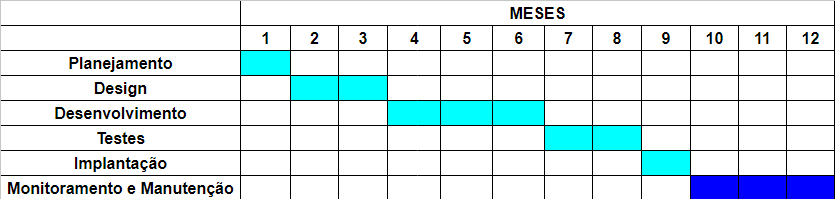
\includegraphics[width=\textwidth]{cronograma.png}
			\caption{Cronograma do Projeto}
			\label{fig:cronograma}
		\end{figure}
		
       \subsection{Alternativas Tecnol\'{o}gicas }
       Ao realizar um estudo de viabilidade para o Sistema de Gerenciamento de Concessionárias de Motos, é fundamental considerar diferentes alternativas tecnológicas que podem ser empregadas para atender aos objetivos do sistema. Essas alternativas podem variar em termos de arquitetura, plataformas, linguagens de programação, bancos de dados e outras tecnologias relevantes. No entanto, a análise de viabilidade não se limita apenas às decisões tecnológicas. Ela abrange uma avaliação holística, incluindo considerações de hardware, software, treinamento, manutenção e outros fatores operacionais.
       
       Aqui, exploraremos algumas das principais alternativas tecnológicas e operacionais a serem consideradas:
       
       \subsubsection{Arquitetura do Sistema}
       
       \begin{itemize}
       	\item \textbf{Arquitetura Cliente-Servidor:} Nesse modelo, o sistema consiste em um servidor central que armazena dados e processa solicitações dos clientes. Os clientes, que podem ser aplicativos web ou móveis, interagem com o servidor para acessar informações e funcionalidades.
       	\item \textbf{Arquitetura em Nuvem:} Utilizar serviços em nuvem, como AWS, Azure ou Google Cloud, oferece escalabilidade e flexibilidade. Isso pode reduzir custos com infraestrutura física e simplificar o gerenciamento de servidores.
       \end{itemize}
       
       \subsubsection{Plataforma de Desenvolvimento}
       
       \begin{itemize}
       	\item \textbf{Desenvolvimento Web:} A criação de um sistema baseado na web é uma escolha comum devido à acessibilidade. Frameworks como Django (Python) e Ruby on Rails (Ruby) podem ser considerados.
       	\item \textbf{Desenvolvimento Móvel:} Se for necessário um aplicativo móvel, é preciso escolher entre desenvolver nativamente (iOS/Android), usar um framework multiplataforma como React Native ou optar por uma PWA (Progressive Web App) que funciona em navegadores móveis.
       \end{itemize}
       
       \subsubsection{Banco de Dados}
       
       \begin{itemize}
       	\item \textbf{Banco de Dados Relacional:} Como o PostgreSQL ou MySQL, é adequado para sistemas que exigem estrutura de dados altamente organizada.
       	\item \textbf{Banco de Dados NoSQL:} Caso o sistema precise lidar com dados não estruturados ou semiestruturados, bancos de dados NoSQL, como MongoDB ou Cassandra, podem ser preferíveis.
       \end{itemize}
       
       \subsubsection{Tecnologias de Front-End}
       
       \begin{itemize}
       	\item \textbf{HTML, CSS e JavaScript:} Essas são as tecnologias fundamentais para desenvolver interfaces de usuário para aplicativos web.
       	\item \textbf{Frameworks Front-End:} Utilizar um framework como React, Angular ou Vue.js pode acelerar o desenvolvimento de interfaces ricas e interativas.
       \end{itemize}
       
       \subsubsection{Segurança}
       
       \begin{itemize}
       	\item \textbf{HTTPS e SSL/TLS:} A segurança é crítica, especialmente ao lidar com dados sensíveis. A implementação de protocolos de segurança, como HTTPS, é essencial.
       	\item \textbf{Autenticação e Autorização:} Mecanismos robustos de autenticação de usuário e controle de acesso devem ser considerados.
       \end{itemize}
       
       \subsubsection{Operacionais}
       
       \begin{itemize}
       	\item \textbf{Hardware e Infraestrutura:} Avaliação e seleção de hardware adequado, servidores, redes e outros recursos de infraestrutura.
       	\item \textbf{Software e Licenças:} Consideração das licenças de software necessárias e custos associados.
       	\item \textbf{Treinamento da Equipe:} Planejamento para treinar a equipe no uso eficaz do sistema.
       	\item \textbf{Manutenção e Suporte:} Estratégias para manter o sistema atualizado, corrigir erros e oferecer suporte técnico.
       	\item \textbf{Estratégia de Backup e Recuperação:} Implementação de práticas para proteger dados e garantir a recuperação em caso de falhas.
       	\item \textbf{Continuidade de Negócios:} Planos para garantir a disponibilidade contínua do sistema, mesmo em situações adversas.
       \end{itemize} 
    
	       \subsection{Or\c{c}amento }
	      \subsubsection{Arquitetura do Sistema}
	\begin{itemize}
		\item \textbf{Arquitetura Cliente-Servidor:} Nesse modelo, o sistema consiste em um servidor central que armazena dados e processa solicitações dos clientes. Os clientes, que podem ser aplicativos web ou móveis, interagem com o servidor para acessar informações e funcionalidades.
		
		\begin{itemize}
			\item \textbf{Orçamento 1 (Cliente-Servidor Local):}
			\begin{itemize}
				\item Hardware de servidor local: R\$ 15.000
				\item Software de servidor: R\$ 5.000
				\item Desenvolvimento de aplicativos cliente: R\$ 20.000
				\item Treinamento da equipe: R\$ 8.000
				\item Manutenção anual: R\$ 6.000
			\end{itemize}
			
			\textbf{Total: R\$ 54.000}
			
			\item \textbf{Orçamento 2 (Cliente-Servidor em Nuvem):}
			\begin{itemize}
				\item Serviços de nuvem (anual): R\$ 25.000
				\item Desenvolvimento de aplicativos cliente: R\$ 20.000
				\item Treinamento da equipe: R\$ 8.000
				\item Manutenção anual: R\$ 6.000
			\end{itemize}
			
			\textbf{Total: R\$ 59.000}
			
			\item \textbf{Orçamento 3 (Híbrido - Local e Nuvem):}
			\begin{itemize}
				\item Hardware de servidor local: R\$ 15.000
				\item Serviços de nuvem (anual): R\$ 15.000
				\item Software de servidor: R\$ 5.000
				\item Desenvolvimento de aplicativos cliente: R\$ 20.000
				\item Treinamento da equipe: R\$ 8.000
				\item Manutenção anual: R\$ 6.000
			\end{itemize}
			
			\textbf{Total: R\$ 69.000}
		\end{itemize}
		
		
		\item \textbf{Arquitetura em Nuvem:} Utilizar serviços em nuvem, como AWS, Azure ou Google Cloud, oferece escalabilidade e flexibilidade. Isso pode reduzir custos com infraestrutura física e simplificar o gerenciamento de servidores.
		
		\begin{itemize}
			\item \textbf{Orçamento 1 (Nuvem Principal):}
			\begin{itemize}
				\item Serviços de nuvem (anual): R\$ 30.000
				\item Desenvolvimento e manutenção: R\$ 25.000
				\item Treinamento da equipe: R\$ 8.000
			\end{itemize}
			
			\textbf{Total: R\$ 63.000}
			
			\item \textbf{Orçamento 2 (Diversificação de Nuvens):}
			\begin{itemize}
				\item Serviços de nuvem (anual - múltiplas plataformas): R\$ 35.000
				\item Desenvolvimento e manutenção: R\$ 25.000
				\item Treinamento da equipe: R\$ 8.000
			\end{itemize}
			
			\textbf{Total: R\$ 68.000}
			
			\item \textbf{Orçamento 3 (Nuvem Híbrida):}
			\begin{itemize}
				\item Serviços de nuvem (anual): R\$ 20.000
				\item Hardware de servidor local: R\$ 10.000
				\item Desenvolvimento e manutenção: R\$ 25.000
				\item Treinamento da equipe: R\$ 8.000
			\end{itemize}
			
			\textbf{Total: R\$ 63.000}
		\end{itemize}
		
	\end{itemize}
	
	\subsubsection{Plataforma de Desenvolvimento}
	\begin{itemize}
		\item \textbf{Desenvolvimento Web:} A criação de um sistema baseado na web é uma escolha comum devido à acessibilidade. Frameworks como Django (Python) e Ruby on Rails (Ruby) podem ser considerados.
		
		\begin{itemize}
			\item \textbf{Orçamento 1 (Django - Python):}
			\begin{itemize}
				\item Desenvolvimento web usando Django: R\$ 40.000
				\item Treinamento da equipe: R\$ 8.000
				\item Manutenção anual: R\$ 10.000
			\end{itemize}
			
			\textbf{Total: R\$ 58.000}
			
			\item \textbf{Orçamento 2 (Ruby on Rails - Ruby):}
			\begin{itemize}
				\item Desenvolvimento web usando Ruby on Rails: R\$ 45.000
				\item Treinamento da equipe: R\$ 8.000
				\item Manutenção anual: R\$ 12.000
			\end{itemize}
			
			\textbf{Total: R\$ 65.000}
			
			\item \textbf{Orçamento 3 (Customizado - PHP):}
			\begin{itemize}
				\item Desenvolvimento web personalizado (PHP): R\$ 35.000
				\item Treinamento da equipe: R\$ 8.000
				\item Manutenção anual: R\$ 8.000
			\end{itemize}
			
			\textbf{Total: R\$ 51.000}
		\end{itemize}
		
		
		\item \textbf{Desenvolvimento Móvel:} Se for necessário um aplicativo móvel, é preciso escolher entre desenvolver nativamente (iOS/Android), usar um framework multiplataforma como React Native ou optar por uma PWA (Progressive Web App) que funciona em navegadores móveis.
		
		\begin{itemize}
			\item \textbf{Orçamento 1 (Desenvolvimento Nativo):}
			\begin{itemize}
				\item Desenvolvimento de aplicativo móvel nativo (iOS/Android): R\$ 60.000
				\item Treinamento da equipe: R\$ 8.000
				\item Manutenção anual: R\$ 15.000
			\end{itemize}
			
			\textbf{Total: R\$ 83.000}
			
			\item \textbf{Orçamento 2 (React Native):}
			\begin{itemize}
				\item Desenvolvimento de aplicativo usando React Native: R\$ 50.000
				\item Treinamento da equipe: R\$ 8.000
				\item Manutenção anual: R\$ 12.000
			\end{itemize}
			
			\textbf{Total: R\$ 70.000}
			
			\item \textbf{Orçamento 3 (PWA - Progressive Web App):}
			\begin{itemize}
				\item Desenvolvimento de PWA: R\$ 45.000
				\item Treinamento da equipe: R\$ 8.000
				\item Manutenção anual: R\$ 10.000
			\end{itemize}
			
			\textbf{Total: R\$ 63.000}
		\end{itemize}
\end{itemize}
		

	\subsubsection{Banco de Dados}
	\begin{itemize}
		\item \textbf{Orçamento 1: PostgreSQL}
		\begin{itemize}
			\item Escolha da Tecnologia: PostgreSQL
			\item Desenvolvimento do Banco de Dados: \$10,000
			\item Otimização de Consultas: \$3,000
			\item Integração com Aplicativo: \$4,000
			\item Backup e Recuperação: \$2,000
			\item Treinamento da Equipe (caso necessário): \$2,500
			\item Manutenção Mensal (opcional): \$1,500
		\end{itemize}
		
		\textbf{Total: \$23,000}
		
		\item \textbf{Orçamento 2: MySQL}
		\begin{itemize}
			\item Escolha da Tecnologia: MySQL
			\item Desenvolvimento do Banco de Dados: \$9,000
			\item Otimização de Consultas: \$2,500
			\item Integração com Aplicativo: \$3,500
			\item Backup e Recuperação: \$1,800
			\item Treinamento da Equipe (caso necessário): \$2,000
			\item Manutenção Mensal (opcional): \$1,200
		\end{itemize}
		
		\textbf{Total: \$19,000}
		
		\item \textbf{Orçamento 3: Banco de Dados NoSQL (MongoDB)}
		\begin{itemize}
			\item Escolha da Tecnologia: MongoDB
			\item Desenvolvimento do Banco de Dados NoSQL: \$12,000
			\item Configuração e Otimização: \$4,000
			\item Integração com Aplicativo: \$3,500
			\item Backup e Recuperação: \$2,500
			\item Treinamento da Equipe (caso necessário): \$2,800
			\item Manutenção Mensal (opcional): \$1,800
		\end{itemize}
		
		\textbf{Total: \$26,800}
	\end{itemize}
	
	
	\subsubsection{Tecnologias de Front-End}
	\begin{itemize}
		\item \textbf{Orçamento 1: Desenvolvimento Front-End Básico}
		\begin{itemize}
			\item Desenvolvimento de Páginas HTML: \$5,000
			\item Estilização com CSS: \$3,000
			\item Programação JavaScript: \$4,000
			\item Integração com Back-End (opcional): \$2,500
			\item Testes e Depuração: \$1,500
			\item Otimização para Dispositivos Móveis: \$2,000
		\end{itemize}
		
		\textbf{Total: \$18,000}
		
		\item \textbf{Orçamento 2: Desenvolvimento Front-End Avançado}
		\begin{itemize}
			\item Desenvolvimento de Páginas HTML Avançadas: \$7,000
			\item Estilização com CSS Avançado e Animações: \$4,500
			\item Programação JavaScript Complexa: \$6,500
			\item Integração com Back-End (opcional): \$3,000
			\item Testes e Depuração Avançados: \$2,500
			\item Otimização para Dispositivos Móveis e SEO: \$3,000
		\end{itemize}
		
		\textbf{Total: \$26,500}
		
		\item \textbf{Orçamento 3: Desenvolvimento Front-End Personalizado}
		\begin{itemize}
			\item Desenvolvimento de Páginas HTML Personalizadas: \$8,000
			\item Estilização Personalizada com CSS: \$5,000
			\item Programação JavaScript Sob Medida: \$7,000
			\item Integração com Back-End Personalizada (opcional): \$4,000
			\item Testes e Depuração Exaustivos: \$2,000
			\item Otimização Avançada para Dispositivos Móveis e SEO: \$3,500
		\end{itemize}
		
		\textbf{Total: \$29,500}
	\end{itemize}
	
	\subsubsection{Segurança}
	\begin{itemize}
		\item \textbf{Orçamento 1: Implementação de HTTPS e SSL/TLS}
		\begin{itemize}
			\item Configuração e Implementação de HTTPS: \$5,000
			\item Configuração e Certificados SSL/TLS: \$3,000
			\item Auditoria de Segurança: \$2,000
		\end{itemize}
		
		\textbf{Total: \$10,000}
		
		\item \textbf{Orçamento 2: Desenvolvimento de Mecanismos de Autenticação e Autorização}
		\begin{itemize}
			\item Implementação de Autenticação: \$6,000
			\item Implementação de Autorização: \$4,000
			\item Testes de Segurança: \$2,500
		\end{itemize}
		
		\textbf{Total: \$12,500}
		
		\item \textbf{Orçamento 3: Segurança Global}
		\begin{itemize}
			\item Implementação de HTTPS e SSL/TLS: \$5,000
			\item Desenvolvimento de Mecanismos de Autenticação e Autorização: \$10,000
			\item Auditoria de Segurança: \$2,000
		\end{itemize}
		
		\textbf{Total: \$17,000}
	\end{itemize}
	
	\subsubsection{Operacionais}
	\begin{itemize}
		\item \textbf{Orçamento 1: Hardware e Infraestrutura}
		\begin{itemize}
			\item Avaliação e Seleção de Hardware: \$10,000
			\item Aquisição de Servidores e Equipamentos: \$25,000
			\item Configuração de Redes e Infraestrutura: \$15,000
		\end{itemize}
		
		\textbf{Total: \$50,000}
		
		\item \textbf{Orçamento 2: Software e Licenças}
		\begin{itemize}
			\item Licenças de Software Necessárias: \$20,000
			\item Aquisição de Software Específico: \$15,000
			\item Custos Mensais de Licenças: \$5,000
		\end{itemize}
		
		\textbf{Total: \$40,000}
		
		\item \textbf{Orçamento 3: Treinamento, Manutenção e Suporte}
		\begin{itemize}
			\item Treinamento da Equipe: \$12,000
			\item Manutenção e Suporte Técnico Anual: \$18,000
			\item Estratégia de Backup e Recuperação: \$8,000
			\item Continuidade de Negócios: \$10,000
		\end{itemize}
		
		\textbf{Total: \$48,000}
	\end{itemize}
	

       \subsection{Resumo e Recomenda\c{c}\~{o}es}

       Considerando todas as análises realizadas até o momento, é fundamental apresentar uma visão clara sobre a viabilidade do sistema de gerenciamento proposto para concessionárias de motos. Este resumo servirá como guia para a tomada de decisões críticas em relação à continuação deste projeto.
       
       \subsubsection{Viabilidade Técnica:}
       
       A análise da viabilidade técnica revela que o Sistema de Gerenciamento de Concessionárias de Motos é tecnicamente viável. A equipe de desenvolvimento possui as habilidades e o conhecimento necessários para implementar com sucesso o sistema. Além disso, as alternativas tecnológicas consideradas, como a arquitetura cliente-servidor, plataforma de desenvolvimento web e banco de dados, são amplamente aceitas e adequadas para atender às necessidades do sistema.
       
       \subsubsection{Viabilidade Financeira:}
       
       A viabilidade financeira do projeto também é positiva. A análise financeira abrange não apenas os custos iniciais de desenvolvimento, mas também os custos em curso, como treinamento da equipe, manutenção, serviços de nuvem e licenças de software. Os benefícios esperados, como aumento das vendas, otimização de processos e maior eficiência operacional, superam os custos associados ao sistema. Portanto, o sistema é viável do ponto de vista financeiro.
       
       \subsubsection{Viabilidade Operacional:}
       
       A viabilidade operacional é uma consideração crucial. Isso inclui a capacidade da equipe de operar o sistema eficientemente, garantir a segurança dos dados, manter a continuidade dos negócios e lidar com situações adversas. A análise mostra que, com a implementação de práticas adequadas de segurança, treinamento contínuo da equipe e planos de contingência, a operação do sistema pode ser realizada com sucesso.
       
       \subsubsection{Recomendação Final:}
       
       Com base nas análises realizadas, é altamente recomendável prosseguir com o desenvolvimento do Sistema de Gerenciamento de Concessionárias de Motos. Este sistema tem o potencial de trazer melhorias significativas nas operações das concessionárias, proporcionando maior eficiência, controle de estoque, gestão de vendas e atendimento ao cliente.
       
       O investimento inicial será compensado pelos benefícios a longo prazo, e a viabilidade técnica, financeira e operacional do projeto está bem fundamentada. No entanto, é essencial que a equipe de desenvolvimento, operações e gerenciamento esteja comprometida e preparada para enfrentar os desafios associados ao projeto.
       
       Em resumo, o Sistema de Gerenciamento de Concessionárias de Motos é uma iniciativa promissora que pode trazer vantagens competitivas para a empresa. Sua implementação deve ser cuidadosamente planejada e executada, com foco na eficiência, segurança e satisfação do cliente.
